%!TEX root = ../main.tex
\section{Introduction}
\label{sec:introduction}
The Internet of Things (IoT) with billions of sensors brought forward the need to redesign existing data management systems.
% 
The main game changer is the massive data production at the edge, in particular from mobile devices that are located \textit{outside} the cloud~\cite{zeuch2020nebulastream}.
%
Gartner predicts that cloud providers will manage 20\% of all edge and mobile computing platforms by 2023, from the current 1\%~\cite{mcarthur2020gartner}.
% \steffen{I don't get this sentence and it reads somehow off}
Recent extensions to the cloud computing paradigm, such as Fog-Cloud~\cite{bonomi2012fog}, Edge Computing~\cite{shi2016edge}, Sensor-Clouds~\cite{yuriyama2010sensor}, and Cloudlets~\cite{satyanarayanan2009case} consider mobile nodes as an integral part of data management systems.
%
Fundamentally, these extensions propose the unification of centralized and immobile nodes in the cloud together with distributed and mobile wireless sensor networks (WSNs). At the same time, intermediate gateway nodes that connect the edge to the cloud are also capable of processing information~\cite{lerner2019cidr, zhang2020gallium}.
% 
However, current approaches assume uninterrupted connectivity to mobile devices, which is seldom the case in today's dynamic and volatile environments such as smart cities~\cite{bonomi2012fog}.
% 
Thus, systems need to incorporate the notion of mobility for data sources and infrastructures into their core design to really enable future IoT applications.

IoT data management concerns the management and processing of data streams, potentially in combination with data at rest, in a heterogeneous distributed environment
 of cloud and mobile edge devices.
One of the main challenges for IoT data management systems is to timely answer user queries that span across cloud and mobile WSN nodes. 
To this end, a system requires real-time knowledge of the underlying topology to keep track of volatile nodes in a scalable manner.
% 
In particular, maintaining a topology that unifies mobile as well as stationary nodes is challenging as nodes connect or disconnect from the system \textit{anytime} and \textit{anywhere} in the network.
% 
At the same time, mobile nodes induce \textit{fluctuations in bandwidth}, \textit{unstable latency}, and \textit{increased  communication overhead}~\cite{li2020beyond}.
% 
The inherent volatility in the topology complicates the deployment and routing decisions within an IoT data management system. 
% 
%Thus, a decision might affect the available bandwidth and latency of other queries.
% 
As a result, one major challenge for an IoT data management system is to determine which nodes and paths provide answers to queries and which of these options induce minimal communication overhead.

\textbf{Motivating Example}
Figure~\ref{fig:problem} 
%\steffen{the figure does not look like a smart city to me as it is much too regular}
shows a simplified view of an IoT installation in a smart city, containing a sink \textInvertedTriangle, gateways 
\textDiamond, and edge devices with sensors \textCircle. The edge devices are attached to mobile phones to keep track of their environment. Multiple gateways, installed at the sides of streets, offer connectivity to the edge devices with one gateway per street. The sink is located at the offices of the data analysis department of the municipality, using their own municipal cloud. The dotted ring indicates the boundary between the edge level (before the gateways) and the municipal infrastructure (gateways and cloud). The ring also indicates the difference in communication methods between nodes. Gateways request information from an edge device, hence they utilize \textit{pull-based} approaches. After gateways acquire values from the edge, they forward it to the municipal cloud by utilizing a \textit{push-based} communication scheme.

Suppose a data analyst wants to send a push notification to edge devices on three different streets. If the device user accepts the notification, the edge device sends sensor data in real time to the cloud. At the same time, the analyst wants to avoid notifying edge devices with low battery. The data analyst thus would issue the following query: \texttt{SELECT * FROM edge\_nodes WHERE battery\_level >= battery\_threshold AND street\_name IN (s\_1,s\_2,s\_3)}.
%
To answer the query, an IoT data management system has to ask all edge devices in \texttt{s\_1, s\_2,} and \texttt{s\_3} about their current battery level, using the closest gateway to the edge device.
%
In Figure~\ref{fig:problem}, \textit{red} routes indicate edge devices that do not have enough battery.
Even though these edge devices should not report back, some systems would still ask them for reporting, even in subsequent queries~\cite{aggarwal2013managing, woo2001transmission}.
% 
In contrast, the \textit{green} route contains a edge device with enough battery and thus information has to move from the yellow edge device to the sink in \textInvertedTriangle.
%
In this scenario, a system needs to communicate and keep track of the yellow edge device as it moves potentially to streets outside of the original query.
At the same time, a system has to reduce communication costs with edge devices that do not have enough battery. 
As a result, the system has to unify a pull-based approach (edge level) with a push-based approach (gateways and upstream) in order to answer queries in different physical partitions of the network. 
% \steffen{push and pull come out of the nowhere and need to be introduced before. This comment is still true as I don't know what they are.}
%

\begin{figure}[t]
        \centering
        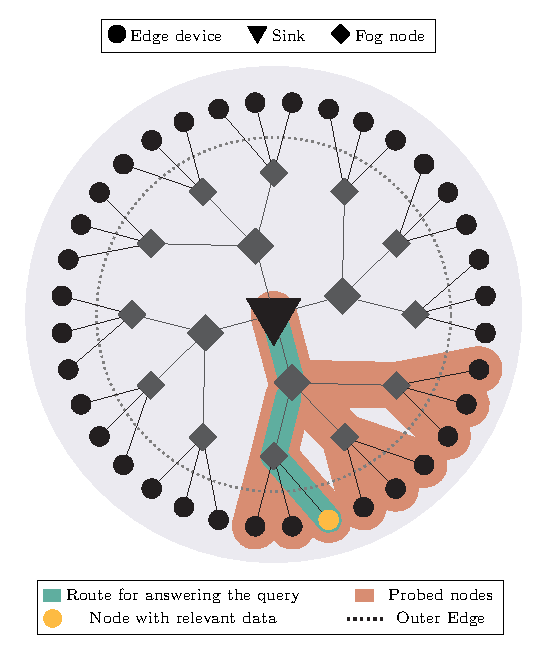
\includegraphics[width=0.4\textwidth]{img/vliot-intro-graphic/tex/intro-fog-topology.pdf}
        \caption{An IoT topology showing edge devices participating in a query. \textit{Red} indicates edge devices that are not relevant but are still probed for values. \textit{Green} indicates vehicles that contain data relevant to the query and have to report their values back.}
        \label{fig:problem}
\end{figure}

\textbf{Contributions}
To enable query processing within a mobile environment, we address the challenges of heterogeneous communication schemes with Rime.
Our solution is a geo-distributed approach for propagating routing information efficiently in an IoT environment. Rime organizes a topology into parent nodes with multiple children nodes, thus forming a hierarchical tree structure over the topology.
% in a topology with minimal overhead, across different physical areas. 
Rime bridges the gap between centralized and mobile approaches by extending the concept of Semantic Routing 
Trees (SRTs)~\cite{madden2005tinydb} from WSNs to the IoT. 
% SRTs are data structures that index information of a node and store it on their \textit{parent}. 
% The parent is responsible of keeping track of its child nodes as well as initiating communication. We talk about SRTs in detail, as well as other core parts of Rime, in Section \ref{sec:background}. 
%
In this paper, we make the following contributions: 
\begin{itemize}
        \item We propose Rime, our approach for efficiently building and maintaining an overview of an IoT topology.
        \item We introduce a novel parent node selection scheme that introduces new nodes to the network with minimal overhead.
        \item We redesign SRTs to use instant communication between parent nodes within an IoT topology.
        \item We evaluate Rime in an emulated IoT network and show that it reduces communication overhead for queries with high index selectivity significantly.
\end{itemize}

We organize the remainder of the paper as follows. In Section~\ref{sec:background}, we provide the necessary background for our work. Then, we propose the core design decisions of Rime in Section~\ref{sec:design} and evaluate them in Section~\ref{sec:evaluation}. After that, we discuss related work in Section~\ref{sec:related-work} and provide an outlook into future work together with our conclusion in Section~\ref{sec:conclusion}.
